\chapter{Planning the design}
\label{ch:planning}

This chapter deals with the initial planning of the design, where the most important factors are considered.

\section{Inspiration}

The PictogramApp application, of which the master project will primarily be based on, allows users to create their own \emph{stories} consisting of an arbitrary number of \emph{scenes}. These concepts can be applied to the new application, though they will be named as \emph{procedures} and \emph{steps} respectively.

(...)

\section{Target groups}

As the requirements reveal, the application is intended for several users. It is therefore important to know who these users may be. For this project, these users are described in form of target groups.

The primary target group will be children and youth at the clinic with ages raging from 5 to 12. The content of the application must therefore be adapted to the target group and be suitable for their age.

The second target group will be the staff at the clinic. This includes physicians, practicioners, consultants, medical assistants and other people working with healthcare.

A third target group is relatives and parents of patients. This group is worth considering as they do have an influence for the patient's stay. In fact, parents contribute to decision-making for most children.

An essential plan when it comes to the design of the application is to let children of the intended age group test it in various stages of its development. Their input is valuable since it can contribute to making the application age-appropriate \autocite{stalberg2016}.

\section{Domain}

The domain of the application is centered around healthcare and treatment of patients.

% Pakkeforløp (...)

Given that the application will be used in a hospital setting, the associated terminology will be extended to the application.

A class diagram of the domain is shown in \autoref{fig:domain1}, illustrating core concepts the application may have to deal with. As some concepts do not have proper English translations, both Norwegian and English names are displayed to avoid confusion.

(...)

% This figure describes ...
% Mer ...

\begin{figure}
    \centering
    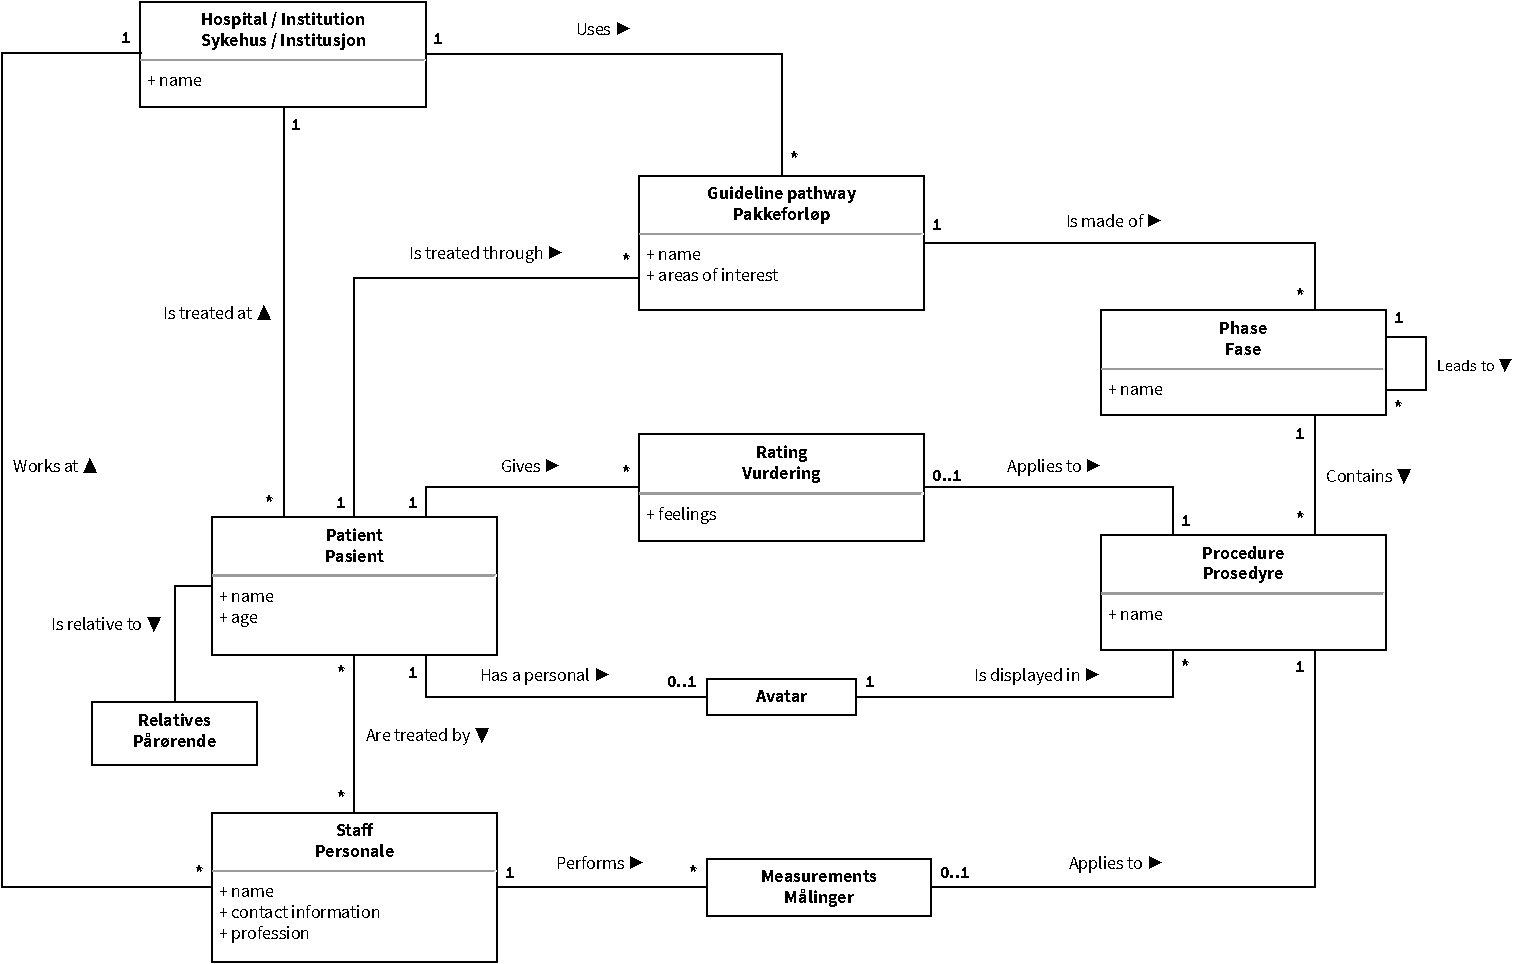
\includegraphics[width=1\textwidth]{domain-model-general.pdf}
    \caption{Domain model showing core concepts}
    \label{fig:domain1}
\end{figure}

The scope of this project will be restricted, involving minimal integration with existing healthcare and journal systems at the Children and Youth Clinic and Haukeland University Hospital. There are not many options for an integration process as of now, and thus any integrations will only be thought of and exact details may be missing.

\section{Requirements}
\label{sec:requirements}

The first step of the interaction design lifecycle is centered around establishing requirements. This involves having a dialog with the client, getting an idea of what they expect and correcting the requirements if they change. \textcite{preece2015} lists out two aims of a requirement activity:

\begin{quote}
    One aim is to understand as much as possible about the users, their activities, and the context of that activity, so the system under development can support them in achieving their goals. Building on this, our second aim is to produce a set of stable requirements that form a sound basis to start designing.

    \raggedleft--- \textcite{preece2015}
\end{quote}

The initial requirements were formed after a meeting with Helgesen and Thorsen. These are divided into functional requirements which describe what the application should do, and non-functional requirements which tell something about constraints of the application and its development. Some of the requirements mentioned here appeared during the design process.

\subsection{Functional requirements}

The Children and Youth Clinic wishes to have an application where the user can view personally targeted procedures. These will feature the user's own personal avatar along with information about an upcoming procedure at the hospital. Afterwards, the user should be able to rate their experience, and if possible, this rating should be reflected when the procedure is shown in retrospect.

(...)

An use case diagram is shown in \autoref{fig:usecases1}. Although some use cases are shared amongst both patient and staff, it may be appropriate to split them across different applications.

\begin{figure}
    \centering
    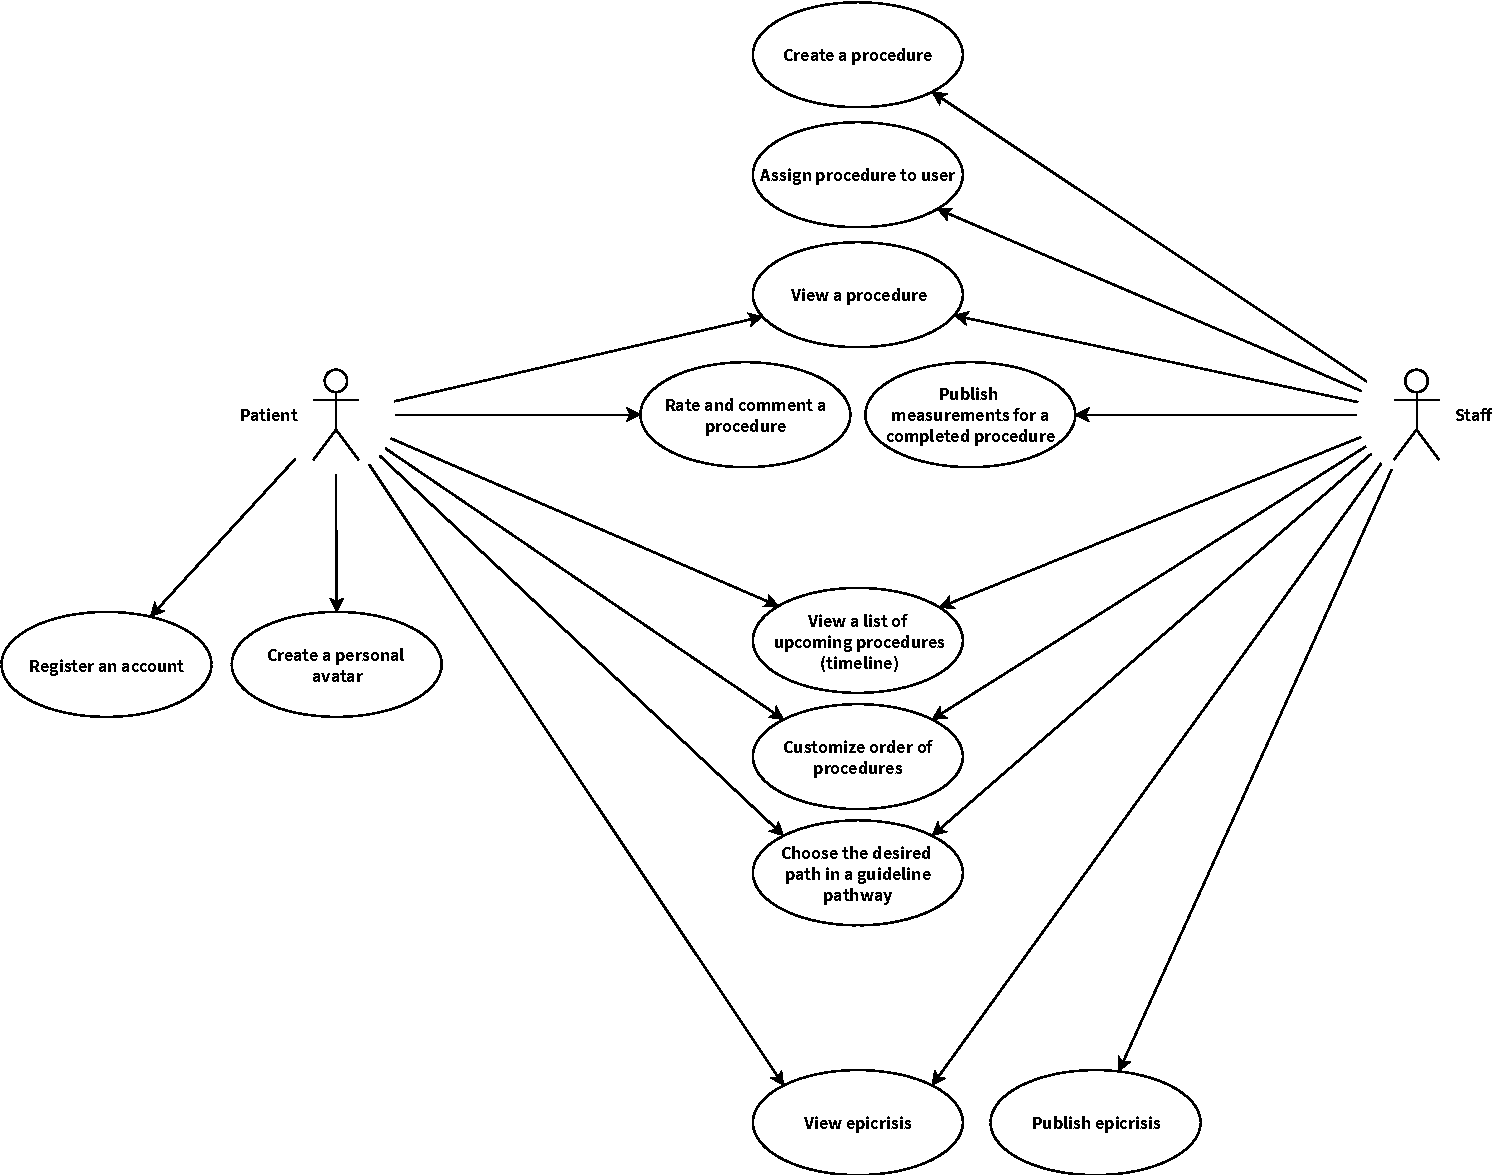
\includegraphics[width=1\textwidth]{use-cases-general.pdf}
    \caption{Use case diagram depicting use cases for a patient and a member of the staff}
    \label{fig:usecases1}
\end{figure}

\subsection{Non-functional requirements}

To begin with, the Children and Youth Clinic expressed that this application is intended to be used on tablets with medium to large screens. There are no requirements regarding which operating systems the software should run on, but the clinic informed that most of their tablets run Windows and Android operating systems.

(...)

% Mer
% - på sykehusets utstyr
% - bærbart
